\documentclass[aps,prd,amsmath,showpacs,amssymb,superscriptaddress,nofootinbib,longbibliography,eqsecnum,preprintnumbers]{revtex4-1}
\usepackage{graphicx}
\usepackage{bm}
\usepackage{amssymb,amsmath}
\usepackage{mathrsfs}
\usepackage{braket} 
\usepackage{latexsym}
\usepackage{color}
\usepackage{float}
\usepackage[normalem]{ulem} 
\usepackage{dcolumn}
\usepackage[colorlinks=true,citecolor=blue,urlcolor=blue]{hyperref}
\usepackage[usenames,dvipsnames]{xcolor}

\allowdisplaybreaks

\newcommand{\odd}{\Psi_{\rm odd}}
\newcommand{\Caltech}{\affiliation{Theoretical Astrophysics 350-17, California Institute of Technology, Pasadena, CA 91125}}
\newcommand{\CITA}{\affiliation{Canadian Institute for Theoretical Astrophysics, 60 St. George Street, Toronto, ON, M5S 3H8 Canada}}
\newcommand{\zach}[1]{\textcolor{ForestGreen}{#1}}
\newcommand{\acs}{\alpha_{\rm CS}}
\newcommand{\bcs}{\beta_{\rm CS}}
\newcommand{\Ssh}{S_{\rm shot}}
\newcommand{\Techo}{T_{\rm echo}}

\begin{document}
\title{Numerical Dynamical Chern Simons Black hole}
%\author{Zachary Mark} \Caltech
\begin{abstract}
We consider a Dynamical Cherns Simons (DCS) black hole in the weakly coupled limit. We represent the DCS black hole as Kerr black hole plus a stationary, axisymmetric perturbation.
We use a pseudospectral method to solve the linearized Einstein Equations and Scalar wave equation governing.
\end{abstract}
\maketitle
\tableofcontents

\section{Wave Equation}
We solve the wave equation 
\begin{align}
\Box \theta =-\rho \label{eq:wave}
\end{align}
on a Kerr background for stationary, axisymmetric (SA) solutions. 

In Boyer-Linquist, coordinates $(t,r,c=\cos\theta,\phi)$, SA solutions are independent of t and $\phi$ and the wave operator separates
\begin{align}
\Sigma \Box \theta= \frac{\partial}{\partial r}\left(\Delta \frac{\partial }{\partial r}\theta\right) + \frac{\partial}{\partial c}\left((1-c^2) \frac{\partial }{\partial c}\theta\right)
\end{align}

As an example we will consider an effective charge density $\rho$ that comes from perturbatively solving the Dynamical-Cherns-Simons (DCS) field equations for black hole solutions in the weakly-coupled regime:
\begin{align}
\rho=*RR =\frac{96M^2arc}{\Sigma^6}(3r^2-a^2c^2)(r^2-3a^2c^2)
\end{align}
where $*RR=R_{\nu \mu\rho\sigma}*R^{\mu\nu\rho\sigma}$ is the Pontryagin density.

We will impose boundary conditions of regularity at the poles $c=\pm 1$ and the horizon $r=r_+$, and that the field vanishes at spatial infinity $\lim_{r\to \infty}\theta= 0$

It is useful to introduce a dimensionless radial coordinate $\eta \in [1,\infty)$ via
\begin{align}
\eta=\frac{r-M}{M\sqrt{1-a^2/M^2}} \leftrightarrow r=M+\eta M\sqrt{1-\frac{a^2}{M^2}}
\end{align}
and write Eq.~\eqref{eq:wave} in the form
\begin{align}
\mathcal{L}\theta=G
\end{align}
where
\begin{align}
\mathcal{L}\theta&=\Sigma \Box\theta \\
&= \frac{\partial}{\partial \eta}\left((\eta^2-1)\frac{\partial }{\partial \eta}\theta\right) + \frac{\partial}{\partial c}\left((1-c^2) \frac{\partial }{\partial c}\theta\right)
\end{align}
and 
\begin{align}
G=-\Sigma \rho=\frac{-96M^2arc}{\Sigma^5}(3r^2-a^2c^2)(r^2-3a^2c^2)
\end{align}

In this form it is clear that the homogeneous solutions to Eq.~\eqref{eq:wave} are products of Legendre functions of $\eta$ and $c$.

We find it convenient to compactify the radial domain, defining
\begin{align}
x=\frac{\eta-L-1}{\eta +L-1} \leftrightarrow \eta=\frac{L(1+x)}{1-x}+1
\end{align}

In terms of derivatives with respect to x, we can write $\mathcal{L}\theta$ as
\begin{align}
\frac{L(1+x)(L(1+x)+2(1-x))(1-x)^2)}{}
\end{align}

\section{Pseudospectral (PS) Method: Algorithm}
My discussion of pseudospectral methods follows Boyd \cite{Boyd99chebyshevand} and Saul Teukolksy's Lecture notes. My implementation is influenced by Leo Stein's pseudospectral code to solve for DCS scalar.

In this section we summarize the algorithm for discretizing a differential equation by representing the solution on a set of collocation points $\{x_i\}$ . The method converges exponentially with the number of grid points if the solution is infinitely differentiable.

Consider the ordinary differential equation for $y(x)$
\begin{align}
\mathcal{L} y = G \label{eq:ODE}
\end{align}
where $\mathcal L$ is a differential operator and $G$ is a source term (that are different than above in general), along with some boundary conditions for y.

Based on the boundary conditions and size of the computational domain, choose a set of N collocation points $\{x_i\}$. 
Approximate y by a degree N-1 polynomial\footnote{Note that sometimes, we refer to $y_N$ as an interpolating polynomial but use a generalization of polynomials such as trigonometric polynomials or rational Chebyshev polynomials} $y_N(x)$ that agree on the collocation points $y(x_i)=y_N(x_i)\equiv y_i$. It is convenient to write the interpolating polynomial as
\begin{align}
y_N(x)=\sum_{i=1}^N y_i C_i(x),
\end{align}
where $C_i(x)$ are the Cardinal functions for the abscissa $\{x_i\}$; the ${C_i}$ are the degree N-1 polynomials obeying $C_i(x_j)=\delta_{ij}$, i.e each one is one on a single grid point and zero on the remaining grid points. A useful explicit construction of $C_i(x)$ is 
\begin{align}
C_i(x)=\prod_{j=1, j\neq i}^N\frac{x-x_j}{x_i-x_j}
\end{align}


The discretized version of the equation $\mathcal{L} y =G$ attempts to approximate the coefficients $y_i$ by imposing $\mathcal{L} y_N(x) =G(x)$ at the collocation points $x_i$, yielding N equations (one for each collocation point) for N unknowns $y_i$. More explicitly
\begin{align}
\mathcal{L} y_N(x_i) =\sum_{n=1}^N \mathcal{L}C_j(x_i)y_j =G(x_i)
\end{align}
which is compactly written as a matrix equation
\begin{align}
&L_{ij}y_j=G_i,& &L_{ij}=\mathcal{L}C_j(x_i),&
&G_i=G(x_i)&
\end{align}

The procedure for implementing boundary conditions depends on whether the boundary conditions are ``numerical'' or ``behavioral''\cite{Boyd99chebyshevand}. 

A numerical boundary condition explicitly sets some combination of $y$ and $y'$ equal to a number, e.g. the Dirichlet condition $y(2)=8$ . There are a few schemes for implementing numerical boundary conditions and we will use the boundary bordering scheme. Consider for example, imposing the Dirichlet condition $y(x_1) =\alpha$. The boundary bordering scheme''  scheme consists of replacing the $L_{1j}y_j=G_1$ equation with the equation $y_1=\alpha$. 

A behaviorial boundary condition specifies that the solution has a particular property, e.g. the solution is regular at $x=a$ or that the solution is periodic. A behavioral condition  doesn't explicitly set y or it's derivative equal to a number. In the next section we will see that behavioral boundary conditions often do not have to be imposed if we choose the abscissa intelligently

% On a related note, in the next section, we will how the approximation in representing the solution $y$ by interpolating polynomial $y_N$ with abscissa $\{x_i\}$ is equivalent to representing $y$ by an exponentially-converging truncated series of spectral basis functions, which will explain the exponential convergence of the numerical method.

To apply the PS algorithm to a PDE such as $\mathcal L \theta(\eta,c)=G(\eta,c)$ we introduce a two dimensional grid $\{(\eta_{i_1}, c_{i_2})\}$ and expand
\begin{align}
\theta(\eta, c) \approx \theta_{N_1N_2}(\eta,c) \equiv \sum_{i_1, i_2 =1}^{N_1,N_2} \theta_{i_1i_2}C^1_{i_1}(\eta)C^2_{i_2}(c)
\end{align}
The 1 indicates that the cardinal functions correspond to the $\eta$ abscissa while the 2 indicates that the cardinal functions correspond to the c abscissa and we label the dummy indices with a 1 or 2 for extra clarity.

In our example, solving $\mathcal L\theta=G$ for the DS scalar,
the discretized differential equation becomes
\begin{align}
L_{i_1j_1i_2j_2}\theta_{j_1j_2}=G_{i_1i_2}, \label{eq:L4}
\end{align}
with 
\begin{align}
L_{i_1j_1i_2j_2}=\left[(\eta_{i_1}^2-1)\frac{\partial^2}{\partial \eta^2}+2\eta_i \frac{\partial}{\partial \eta}+(1-c_{i_2}^2)\frac{\partial^2}{\partial c^2}-2c_{i_2}\frac{\partial }{\partial c}\right]C^1_{j_1}(\eta_{i_1})C^2_{j_2}(c_{i_2})
\end{align}

For the results, presented in this paper, I assembled L by using the formula for derivatives of the cardinal functions, known as differentiation matrices, presented in Boyd \cite{Boyd99chebyshevand} (correcting for the errors mentioned in the errata). I used Mathematica's LinearSolve routine to solve the matrix equations. The results are in agreement with Leo's code which uses a slightly different implementation of the pseudospectral method that relies on separation of variables.

\section{Pseudospectral Method: Theory}
In this section we explain why the pseudospectral (PS) algorithm is exponentially convergent with the number of grid points N, justify our claim about behavioral boundary conditions, and in the process show how the psuedospectral algorithm presented above is equivalent to a spectral Galerkin method.

\subsection{Spectral, Galerkin Method}
Consider again the ordinary differential equation for $y(x)$
\begin{align}
\mathcal{L} y = G \label{eq:ODE}
\end{align}
where $\mathcal L$ is a differential operator and $G$ is a source term.

Choose a complete set of functions ${\phi_n(x)}$, known as the spectral basis, and expand $y$ in this basis
\begin{align}
y(x)=\sum_{n=1}^\infty\tilde y_n\phi_n(x)
\end{align}

We choose the spectral basis to corresponding to the eigenfunctions of a Sturm-Louiville system,
\begin{align}
&\frac{d}{dx}\left[p(x)\frac{d\phi_n(x)}{dx}\right]+(\lambda_n w(x)-q(x))\phi_n(x)=0,& &x\in[a,b]
\end{align}
with $p,q,w\geq 0$, along with boundary conditions. If $\rho(a)\neq 0$ and $\rho(b)\neq 0$, the system is regular and homogenous mixed boundary conditions are imposed at each boundary $x=a$ and $x=b$. If $p(a)=p(b)=0$, the system is singular and the boundary conditions are taken to be regularity.

The eigenfunctions $\phi_n$ are orthonormal with the weight function $w(x)$,
\begin{align}
(\phi_m,\phi_n)\equiv \int_a^b\phi_m(x)\phi_n(x)w(x)dx =\delta_{mn}
\end{align}
and complete. Further, if $y$ also obeys the same boundary conditions as the Sturm-Louivelle system and if y is infinitely differentiable , the expansion
\begin{align}
y(x)=\sum_{n=1}^\infty \tilde y_n \phi_n(x)
\end{align}
converges exponentially, i.e $\tilde y_n \ll 1/n^a$ as $n\to \infty$ for all positive values of a. 

This means that we can truncate the expansion 
\begin{align}
y\approx Y_N(x)=\sum_{n=1}^N\tilde y_n\phi_n(x)
\end{align}
and only experience an exponentially converging error $|y-Y_N|$.

Now consider the following Galerkin, spectral scheme for numerical solving the differential equation $z\equiv \mathcal L y-G=0$. Approximate the solution with the truncated spectral expansion $y(x)\approx Y_N(x)$ and solve for the N spectral coefficients ${\tilde y_i}$ by imposing the N Galerkin conditions $\tilde z_n\equiv (\phi_n, z)=0$ for $n=1,..., N$. 

There are three places errors creep into this scheme. 
There is the truncation error (using the language of Boyd \cite{Boyd99chebyshevand}) in approximating $y$ by $Y_n$. As we just discussed this error exponentially vanishes with N.
There is a discretization error in approximating $\mathcal L y$ with $\mathcal L Y_n$, e.g.
\begin{align}
|\mathcal L y -\mathcal L Y_n|=\left|\sum_{n=N+1}^\infty \tilde y_n\mathcal L \phi_n(x)\right|,
\end{align}
which also vanishes exponentially with $N$. 
Finally there is another source of discretization error arising from only setting $\tilde z_n =0$ for $n=1,..N$. This error is
\begin{align}
\left|z-\sum_{n=1}^N\tilde z_n \phi_n(x)\right|=\sum_{n=N+1}^\infty \tilde z_n \phi_n(x)
\end{align}
and also goes to zero exponentially as $N\to \infty$ if $y$ is infinitely differentiable (since this implies that $\mathcal{L} y-G$ is infinitely differentiable.
Thus the total error in the Galerkin, spectral scheme goes to zero exponentially as $N\to \infty$.

\subsection{Relation to Pseudospectral Method}

For a given choice of spectral basis $\{\phi_n\}$, the PS algorithm above is equivalent to the Galerkin, spectral scheme, modulo terms with vanish exponentially as $N\to \infty$ if the collocation points $\{x_i\}$ are chosen correctly.

Recall the Gaussian quadrature integration rule for approximating an integral with N sample points
\begin{align}
\int_a^bI(x)w(x)dx\approx \sum_{i=1}^N w_i I_i,
\end{align}
where $w(x)$ is an integration weight, $w_i$ are weights for the integration rule (unrelated to $w(x)$), $x_i$ are the sample grid points, and $I_i=I(x_i)$. The N weights $w_i$ and N grid points $x_i$ are fixed by the 2N conditions that the integration rule be exact when $I(x)$ is a polynomial of degree 2N-1 or less. In general there are two choices of grid points and weights that satisfy this condition. The Gauss-Chebyshev abscissa consist of points on the interior of the domain $[a,b]$ while the Gauss-Lobatto abscissa include the endpoints of the domain $[a,b]$. Note that Gaussian quadruature integration can be easily generalized to a procedure that fixes the $w_i$ and $x_i$ by demanding the rule be exact on some other $2N-1$ dimensional vector space of polynomials. This is the case for the Gaussian quadrature associated with the trigonometric polynomials.

The Galerkin, spectral method using a spectral basis $\{\phi_n\}$ is equivalent (for infinitely differentiable functions) to the PS method, modulo exponentially vanishing terms, if the abscissa $\{x_i\}$ for the PS method are chosen to be the gaussian quadrature weights associated with $\{\phi_n\}$.
%Note that in order to regard the spectral basis $\phi_n(x)$ as polynomial, it is sometimes necessary to map view them as functions on another domain , i.e the Trignonometric polynomials. \zach{Work through this example.}

To see this, first note that the true spectral coefficients $\tilde y_n=(\phi_n,y)$, which are computed in the spectral Galerkin method, can be obtained from the grid point samples $y_i$ with an exponentially converging (with N) error. Denote the Gaussian quadrature evaluation of the product $(f,g)$ with
\begin{align}
(f,g)_G\equiv \sum_{i=1}^N f_ig_iw_i.
\end{align}
Then we have,
\begin{align}
\tilde y_m&=\left(\phi_m, y\right) \nonumber \\
&=\left(\phi_m, \sum_{n=1}^N\tilde y_n \phi_n\right) + \left(\phi_m, \sum_{n=N+1}^\infty\tilde y_n \phi_n\right) \nonumber \\
&\approx \left(\phi_m, \sum_{n=1}^N\tilde y_n \phi_n\right) \nonumber \\
&=\left(\phi_m, \sum_{n=1}^N\tilde y_n \phi_n\right)_G \nonumber \\
&\approx \left(\phi_m, \sum_{n=1}^N\tilde y_n \phi_n\right)_G +\left(\phi_m, \sum_{n=N+1}^\infty\tilde y_n \phi_n\right)_G \nonumber \\
&=\left(\phi_m, y\right)_G \nonumber \\
&=\sum_{i=1}^\infty w_i \phi_m(x_i)y_i,
\end{align}
where whenever we used the approximate equality we dropped exponentially vanishing terms as $N\to \infty$ and we have repeatedly used the fact that gaussian quadrature integration is exact for polynomialso degree 2N-1 or less. This can be summarized by a matrix relation between the spectral coefficients and the grid space values
\begin{align}
&\tilde y_i=M_{ij}y_j,& &M_{ij}=\phi_i(x_j)w_j&.
\end{align}
Next note, by the same reasoning, the spectral coefficients $\tilde z_n$ of $z=\mathcal L y-G$ can be approximated by the values $z_i=z(x_i)$ on the collocation grid
\begin{align}
\tilde z_i=M_{ij}z_j,
\end{align}
so the imposition of the N Galerkin conditions $\tilde z_i=0$ for $i=1,...,N$ is equivalent to the imposition of the N conditions $z_i=0$ on the grid. 

Thus the two methods are equivalent for infinitely differentiable functions since they impose the same conditions and they solve for the same information. This means that the PS method is also exponentially convergent.

\section{Boundary Conditions}

To implement a behaviorial boundary condition, such as regularity at a boundary or periodicity, simply choose basis functions $\{\phi_n\}$ that satisfy the same condition. 
Then, 
%provided that the spectral coefficients $\tilde y_n$ produced by the algorithm make the sum $\sum_{n=1}^N \tilde y_n \phi_n$ converge, 
the sum $y=\sum_{n=1}^\infty \tilde y_n \phi_n$ will manifestly satisfy the same condition. Thus if the basis is chosen intelligently, nothing needs to be done by the programmer when implementing a behavioral boundary condition. This justifies our earlier claim.

To implement a numerical boundary, there are two available methods. For a boundary condition that occurs at the first or the last grid point, the boundary bordering scheme replaces the equation corresponding to the first or last grid point with the boundary condition. (\zach{zach: Does this scheme affect the exponential convergence of the method}) The basis-function recombination scheme involves defining a new dependent variable $a(y)$ that obeys a homogenous boundary condition and then redefining the spectral basis so that all of the basis functions obey this boundary condition. We do not use basis recombination in this paper.


% by imposing the the differential equation at a set of N colocation points ${x_j}$, resulting in N equations
% \begin{align}
% \sum_{j=1}^N\tilde y_j \mathcal L \phi_n(x_i) =G(x_j),
% \end{align}
% Where
% The optimal choice of colocations points is inherited from the choice of basis functions

\section{Scalar Results}
We solve the scalar equations on the compactified $(x,c)\in((-1,1),(-1,1))$ domain.
We use the Gauss-Lobotto grid (including endpoints) corresponding to the Chebyshev Polynomials for the radial x direction and the Gauss-Lobotto grid (including endpoints) corresponding to the Legendre Polynomials for the angular direction. We implement the behavior boundary conditions of regularity at $x=-1$, $c=\pm$ by doing nothing. We implement the numerical boundary condition at $x=1$ that $\theta =0$ with the boundary bordering method.

% We solve for the DCS scalar by solving
% \begin{align}
% \mathcal{L}\theta(\eta,c) =G(\eta, c)
% \end{align}
% using three variations of PS method.

% \subsection{Boundary Bordering}

% \subsubsection{Gauss-Lobatto Radial Grid}
% We use the Gauss-Lobatto (including endpoints) angular grid $\{c_i\}$ corresponding to the Legendre polynomials, i.e (from Boyd)
% \begin{align}
% c_i = -1, 1, \; \text{and the $N_2-1$ roots of }\; \frac{dP_{N_2}}{dc}.
% \end{align}
% We use $\{C^2_i(c)\}$ to denote the angular cardinal functions corresponding to this grid.

% For the radial grid $\{\eta_i\}$ we use the Gauss-Lobatto grid (including endpoints) corresponding to the rational Chebyshev polynomials. A rational Chebyshev function $TL_n(\eta)=$ is a Chebyshev polynomial that has been mapped to the interval $\eta \in[1,\infty)$ with $x=\frac{\eta -L-1}{\eta+L-1}$, i.e $TL_n(\eta)=T_n(x(\eta))$. The rational Chebyshev's have a free parameter L defining the the rescaling of the unit interval to the semi-infinite interval; ideally the results should be insensitive to the choice of L, provided it is not too far from it's optimal value. The results that we show use $L=1$.
% (\zach{ZM:I'm not sure that I am using standard notation for the rational Chebyshev's here.}) The gaussian quadrature abscissa for the rational Chebyshev functions are simply the abscissa for the Chebyshev polynomials
% \begin{align}
% &x_i=\cos\left(\frac{\pi i}{N_1}\right),& &i=0,..,N_1&.
% \end{align} mapped to the interval $[1,\infty)$ using $\eta(x)$.
% We use a 1 superscript to denote the cardinal functions $\{C_i^1(\eta)\}$ for the radial grid. Note that the cardinal functions for the rational Chebyshevs are the cardinal functions for the Chebyshev's mapped to the domain $\eta \in [1,\infty)$ and hence are not polynomials in $\eta$.
% Note that this entire procedure is equivalent to mapping the problem to a compact radial domain with $\eta =\frac{L(1+x)}{1-x}+1$.

% With these choices, we represent the scalar with an interpolating polynomial
% \begin{align}
% \theta \approx \sum_{i_1=0 i_2=0}^{N_1, N_2}\theta_{i_1 i_2}C^1_{i_1}(\eta)C^2_{i_2}(c).
% \end{align}
% Note following the convention of Boyd\cite{Boyd99chebyshevand}, for the Gauss-Lobatto grid, we shift our convention to start the labeling of the Cardinal functions and grid at $i_1=0$ and $i_2=0$ so this representation contains $N=(N_1+1)(N_2+1)$ grid points.


% The Legendre basis functions are regular, so we do not have to do anything to implement the behavioral boundary condition of regularity at the poles $c=\pm 1$ other than check that the solution converges. Note that the Sturm-Louiville problem associated with the Legendre polynomials  also has boundary conditions of regularity at the poles, so we get the exponential convergence of the truncated spectral expansion for the solution.

% To impose the behavioral radial boundary condition of regularity on the horizon, we also do not do anything other than check the convergence of the solution. Note that the Sturm-Louiville problem associated with the Chebyshev polynomials also has boundary conditions of regularity at the poles, so we get the exponential convergence of the truncated spectral expansion for the solution (\zach{ZM:I need to provide more details here since I think there are subtlies about the infinite interval discussed in Boyd}).

% To impose the numerical boundary condition $\lim_{\eta \to \infty}=0$, we use the boundary bordering procedure. The grid point $\eta_0$ corresponds to $\eta =\infty$ with the definition of the Gauss-Lobatto grid for the rational Chebyshev's. Hence we replace the $i_1=0, j_1$ equations in Eq.~\eqref{eq:L4} with the equations $\theta_{0,j_1}=0$. Since this is trivial solved and substituted back into the rest of the matrix, in practice, this implementation just calls for us to drop the equation corresponding to the $i_1=0$ grid points and the variables $\theta_{0,j_1}$.

% \begin{figure}[t]
% 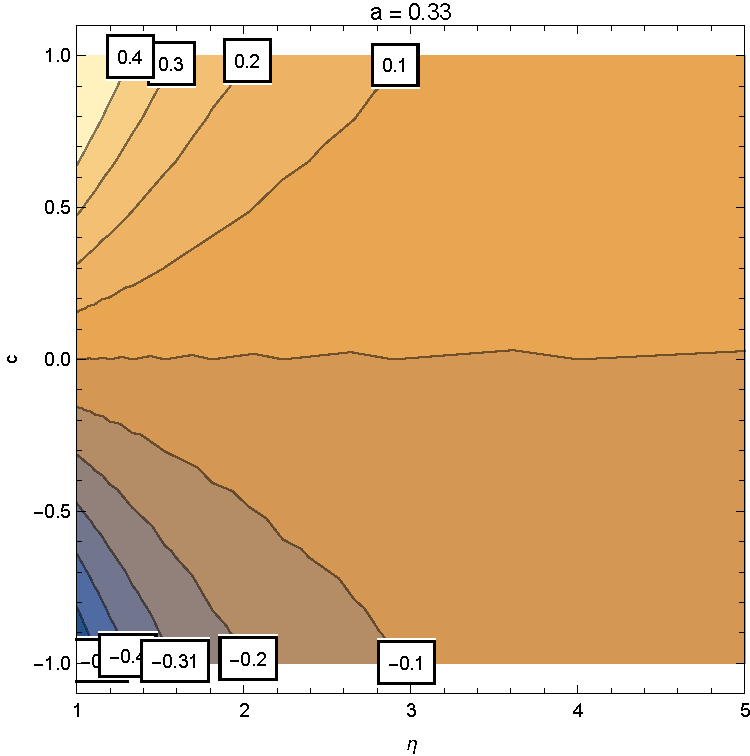
\includegraphics[width =0.3\columnwidth]{a33}
% 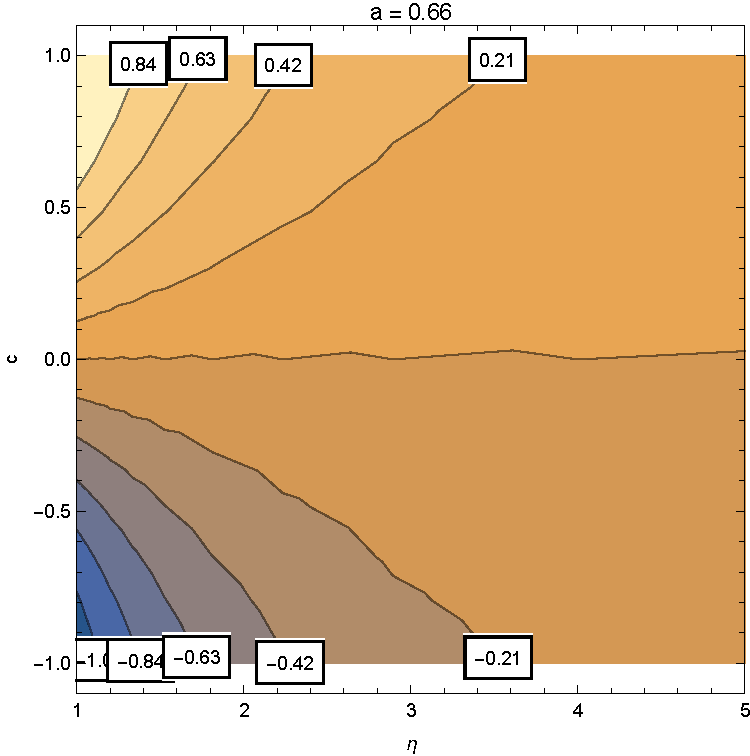
\includegraphics[width =0.3\columnwidth]{a66}
% 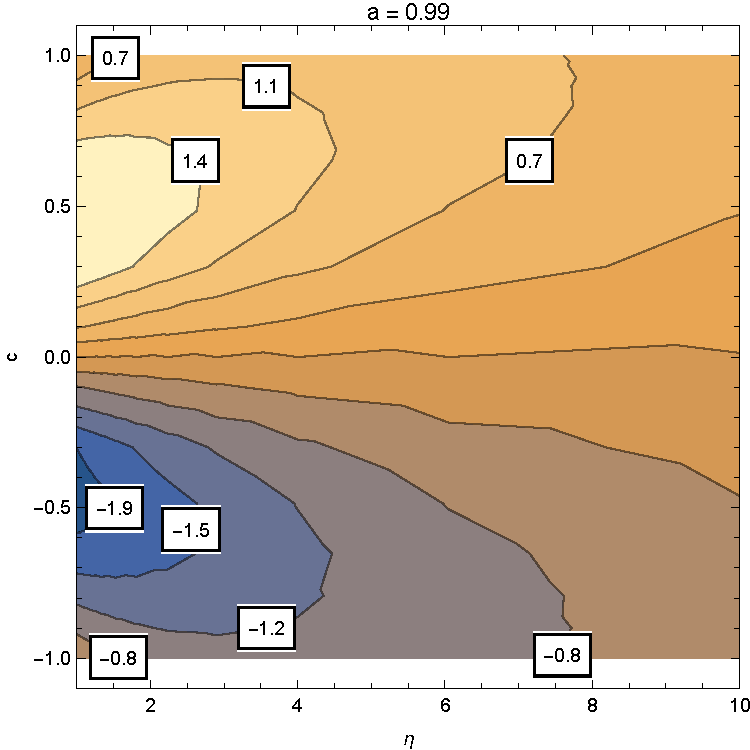
\includegraphics[width =0.3 \columnwidth]{a99}
% \caption{From left to right, the DCS scalar $\theta(\eta,c)$ for $a=0.33M$, $a=0.66M$, $a=0.99M$ using the PS code that doesn't explicitly enforce antisymmetry.
% }
% \label{fig:BB}
% \end{figure}

% Figure \ref{fig:BB} shows contour plots of the scalar produced with $N_1=15$, $N_2=15$, and $L=1$ for three values of a.

% \begin{figure}[t]
% 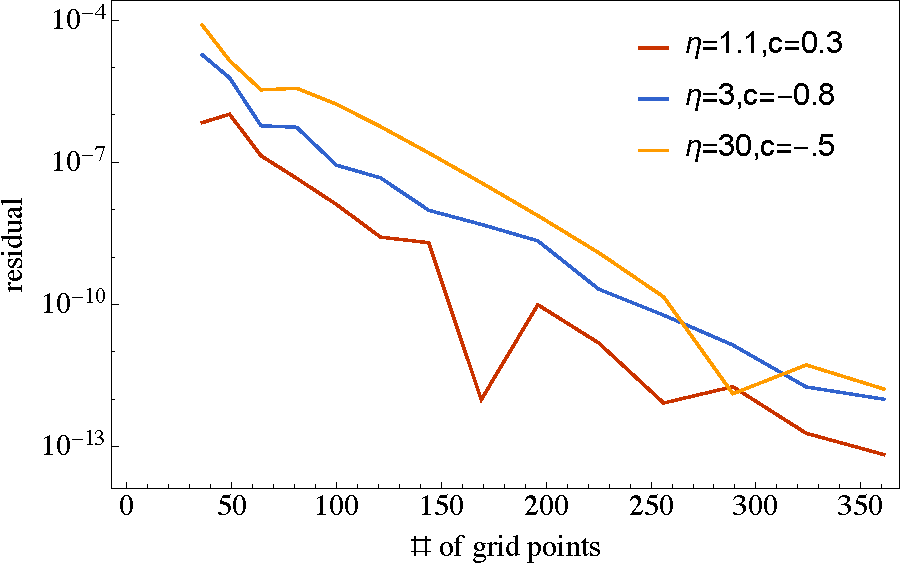
\includegraphics[width =0.9\columnwidth]{BBscalingplot}
% \caption{The residual in the solution with N grid points with the solution withe 420 gridpoints (the finest solution resolution solution computed). These results are for the PS code that doesn't explicitly enforce antisymmetry.
% }
% \label{fig:BBscaling}
% \end{figure}

% Figure \ref{fig:BBscaling} shows the convergence of the result for several different positions for $a=0.2$. The residual of the solution with N gridpoints is defined as as the absolute value of the difference of the solution with N grid points and the solution with 420 grid points (the finest resolution that I chose to compute, although I could easily have gone with even finer resolution). Note the exponential convergence

\section{Metric Perturbations}
\subsection{Equations}
We use numerically convenient variables (for implementing the boundary conditions) $z^{\bar a}=\{\tilde Y, \tilde h_{tt}, \tilde h_{\phi\phi}, \tilde h_{t\phi} \}$ with
\begin{align}
\tilde Y&=\frac{\Delta}{r^2}Y \nonumber \\
\tilde h_{tt}&=r h_{tt} \nonumber \\
\tilde h_{\phi\phi}&=\frac{1}{r^2(1-c^2)}h_{\phi\phi}
\nonumber \\
\tilde h_{t \phi}&=\frac{r}{1-c^2}h_{t\phi}
\end{align}

We index the four evolution equations with barred capitol latin letters$\bar A={+,tt,pp,tp}$ and write the four evoluion equations as
\begin{align}
L_{\bar A}[z]=A_{\bar A \bar a AB}\partial_{A}\partial_{B}z^{\bar a}+B_{\bar A \bar a A}\partial_{A}z^{\bar a}
+C_{\bar A \bar a }z^{\bar a}
\end{align}

\subsection{Discretization}
We discretize $L_{\bar A}$ as 
\begin{align}
&L_{\bar A}[z]\to L_{\bar A \bar a i_1 j_1 i_2 j_2}z_{\bar a j_1 j_2}
\nonumber \\
&=\left[A_{\bar A \bar b ABi_1k_1i_2k_2}\partial_{\bar b \bar c k_1 \ell_1k_2\ell_2A}\partial_{\bar c\bar a \ell_1 j_1\ell_2j_2B}
+B_{\bar A \bar b Ai_1k_1i_2k_2}\partial_{\bar b \bar a k_1j_1k_2j_2A}
+C_{\bar A\bar a i_1 j_1 i_2 j_2}
\right]z_{\bar a j_1 j_2}
\end{align}
where the discretized potentials are defined as 
\begin{align}
&A_{\bar A \bar b ABi_1k_1i_2k_2}=
A_{\bar A\bar b AB}(x^{i_1},c^{i_2})\delta_{i_1j_1}\delta_{i_2j_2}, \nonumber \\
& \text{etc. for B and C,}
\end{align}
and the discretized derivative operators are defined as the appropriate combinations of identity matrices and differentiation matrices $D^1_{i_1j_1}$ and $D^2_{i_2 j_2}$ for the radial and angular domains
\begin{align}
&\partial_{\bar b \bar c k_1 \ell_1k_2\ell_2 x}=D^1_{k_1 \ell_1}\delta_{k_2\ell_2}\delta_{\bar b \bar c}\nonumber \\
&\partial_{\bar b \bar c k_1 \ell_1k_2\ell_2 c}=D^2_{k_2 \ell_2}\delta_{k_1\ell_1}\delta_{\bar b \bar c}\nonumber \\
\end{align}
Note that implementing these definitions exactly results in larger matrix computations than necessary since many of the matrices are very sparse (as they contain tensor products with one or two identity matrices). Right now, the mathematica code implements these definitions exactly (for the ease of the programmer) but represents them with Mathematica's sparse array object to speed computations. Also note that to construct L, it is useful to take advantage of mathematica's TensorContract, Transpose, and TensorProduct operations, as opposed to using functions like sum and table.






 
\bibliography{QNMModelRefs.bib}

\end{document}
